%---------------------------------------------------------------------------------------------------
% Voreinstellungen (Layout, neue Befehle, etc.)
%---------------------------------------------------------------------------------------------------

%---------------------------------------------------------------------------------------------------
% Einstellungen
% (gelten nur in Zusammenarbeit mit pdflatex)
%---------------------------------------------------------------------------------------------------
\documentclass[
  pagesize,	                                           % flexible Auswahl des Papierformats
  a4paper,  	                                         % DIN A4
  oneside,    	                                       % einseitiger Druck
  BCOR5mm,      	                                     % Bindungskorrektur
  headsepline,                                         % Strich unter der Kopfzeile
  12pt,                                                % 12pt Schriftgr��e
	halfparskip,                                         % Europ�ischer Satz: Abstand zwischen Abs�tzen
	abstracton,																					 % Spezielle Formatierung, die erlaubt, dass die
																											 % Zusammenfassung vor dem Inhaltsverzeichnis steht
	%draft,																							 % Es handelt sich um eine Vorabversion	
	final,																							 % Es handelt sich um die endg�ltige Version
	liststotoc,																					 % Tabellen- und Abbildungsverzeichnis im 																																 % Inhaltsverzeichnis
	idxtotoc,																						 % Index im Inhaltsverzeichnis	
  bibtotoc,                                            % Literaturverzeichnis im Inhaltsverzeichnis  
]{scrreprt}                                            % KOMA-Scriptklasse Report

%---------------------------------------------------------------------------------------------------
\usepackage[english,ngerman]{babel}                    % deutsche Trennmuster
\usepackage[T1]{fontenc}                               % EC-Schriften, Trennstellen nach Umlauten
\usepackage[latin1]{inputenc}                          % direkte Umlauteingabe (� statt "a)
                                                       % latin1/latin9 f�r unixoide Systeme
                                                       % (latin1 ist auch unter Win verwendbar)
                                                       % ansinew f�r Windows
                                                       % applemac Macs
                                                       % cp850 OS/2
\usepackage{times}              											 % Schriften Paket
\usepackage{array,ragged2e} 													 % Wichtig f�r Abstandsformatierung

%---------------------------------------------------------------------------------------------------
\usepackage{cmbright}                                  % serifenlose Schrift als Standard
                                                       % + alle f�r TeX ben�tigten mathematischen
                                                       %   Schriften einschlie�lich der AMS-Symbole
\usepackage[scaled=.90]{helvet}                        % skalierte Helvetica als \sfdefault
\usepackage{courier}                                   % Courier als \ttdefault

%---------------------------------------------------------------------------------------------------
\usepackage[automark]{scrpage2}                        % Anpassung der Kopf- und Fu�zeilen
\usepackage{xspace}                                    % Korrekter Leerraum nach Befehlsdefinitionen
\usepackage{setspace}																	 % Dieses Package brauchen wir f�r den 				
\usepackage[pdftex]{graphicx}
\usepackage[absolute,overlay]{textpos}         
\usepackage[final]{pdfpages}																											 % anderthalbzeiligen Abstand.
\usepackage{natbib}                                    % Neuimplementierung des \cite-Kommandos
\usepackage{bibgerm}       											       % Deutsche Bezeichnungen
\usepackage[absolute]{textpos}                         % placing boxes at absolute positions
\usepackage[final]{pdfpages}                           % include pages of external PDF documents
\usepackage{tabularx}                                  % Spaltenbreite bis zur Seitenbreite dehnen
\usepackage{makeidx}
\usepackage{listings}													% Paket zur Erstellung eines Stichwortverzeichnisses
\makeindex																						 % Automatische Erstellung des Stichwortverzeichnis
\usepackage[intoc,
						english,
						prefix]{nomencl}
\makenomenclature

%---------------------------------------------------------------------------------------------------
 \usepackage{graphicx}                                 % Zur Einbindung von PDF-Bildern
 \usepackage[colorlinks,															 % Einstellen und Laden des Hyperref-Pakets
	pdftex,
	bookmarks,
	bookmarksopen=false,
	bookmarksnumbered,
	citecolor=blue,
	linkcolor=blue,
	urlcolor=blue,
	filecolor=blue,
	linktocpage,
  pdfstartview=Fit,                                  % startet mit Ganzseitenanzeige    
	pdfsubject={Multiagentensystemgest�tzte Clusteranalyse},
	pdftitle={Diplomarbeit im Fachbereich Elektrotechnik \& Informatik an der HAW-Hamburg},
	pdfauthor={Bj�rn Jensen, http://www.mirou.de}]{hyperref}
 \pdfcompresslevel=9
 
%---------------------------------------------------------------------------------------------------
% Inhaltsverzeichnis und Abschnittnummerierung
%---------------------------------------------------------------------------------------------------
\setcounter{secnumdepth}{2}   % Ich habe recht kurze Kapitel. Die sollen nicht durchnummeriert sein.
\setcounter{tocdepth}{2}

%---------------------------------------------------------------------------------------------------
% Abbildungsverzeichnis
%---------------------------------------------------------------------------------------------------
\graphicspath{{graphics/}}

%---------------------------------------------------------------------------------------------------
% Kopf- und Fu�zeilen
%---------------------------------------------------------------------------------------------------
\pagestyle{scrheadings}
\clearscrheadings
\clearscrplain
\clearscrheadfoot
\ohead{\pagemark}
\ihead{\headmark}

%---------------------------------------------------------------------------------------------------
% Neue Befehle
%---------------------------------------------------------------------------------------------------
%---------------------------------------------------------------------------------------------------
% Neue Befehle
%---------------------------------------------------------------------------------------------------

%---------------------------------------------------------------------------------------------------
% Umbenennen des Symbolverzeichnisses
%---------------------------------------------------------------------------------------------------
\renewcommand{\nomname}{Glossar}				% Das Symbolverzeichnis heisst nun "Glossar"
\renewcommand{\nomlabel}[1]{						% Die zu erkl�renden Begriffe sind nun fett hervorgehoben
	\hfil \textbf{#1} \hfil
}

%---------------------------------------------------------------------------------------------------
% Ein paar ganz n�tzliche Befehle von Lars M�hlmann
%---------------------------------------------------------------------------------------------------
%f�r Kommentare 
\newcommand{\colb}{\color{green}}
\newcommand{\colbl}{\color{black}}

%---------------------------------------------------------------------------------------------------
% Befehle zum Erstellen des Index
% \addIndexEntry{Eintrag in den Index}
% \addSubIndexEntry{Eintrag in den Index}{Eintrag des �bergeordneten Eintrags}
%---------------------------------------------------------------------------------------------------
\newcommand{\addIndexEntry}[1]{#1\index{#1}}
\newcommand{\addSubIndexEntry}[2]{#1\index{#2!#1}}

%---------------------------------------------------------------------------------------------------
% LaTeX in eigenem Font
%---------------------------------------------------------------------------------------------------
\newcommand{\myLatex}{
	{\rmfamily\LaTeX\xspace}
}

%---------------------------------------------------------------------------------------------------
% Befehl zum Erstellen und Hervorheben eines Zitats
% Parameter:
% 1. Zitat
% 2. Author
% 3. Quelle
%---------------------------------------------------------------------------------------------------
\newcommand{\myCitation}[3]{
	\begin{flushright}
	\begin{minipage}{.4\linewidth}
		\footnotesize\rmfamily\itshape 
		#1 \\
		\RaggedLeft #2 \\
		#3
	\end{minipage}
	\end{flushright}
	\nobreakspace
}

%---------------------------------------------------------------------------------------------------
% Erstellung von Deckblatt (Seite 1) und Titelblatt (Seite 2)
%---------------------------------------------------------------------------------------------------
\newcommand{\createCoverAndTitlePage}[7]{
	\createCover{#1}{#2}{#3}{#4}
	\createTitlePage{#1}{#2}{#3}{#4}{#5}{#6}{#7}
}

%---------------------------------------------------------------------------------------------------
% Erstellung von Deckblatt (Seite 1) 
% Anwendung:
% \createCover{Art der Arbeit}{Typ der Arbeit}{Autor}{Titel}
%---------------------------------------------------------------------------------------------------
\newcommand{\createCover}[4]{
	\thispagestyle{empty}
	\begin{titlepage}

	\setlength{\TPHorizModule}{1mm}
	\setlength{\TPVertModule}{1mm}
	\textblockorigin{0mm}{0mm} % start everything near the top-left corner

	% Art der Arbeit
	\begin{textblock}{111}(83,115)
		\begin{minipage}[c][1,78cm][c]{11,09cm}		
  		\fontsize{22pt}{20pt}
  		\selectfont
  		\begin{center}
  		#1#2
  		\end{center}
		\end{minipage}
	\end{textblock}

	% Name & Titel
	\begin{textblock}{111}(83,131)
		\begin{minipage}[c][4,81cm][t]{11,09cm}	
		\linespread{1.2}	
    		\fontsize{16pt}{14pt}    
    		\selectfont
    		\begin{center}
    			#3 \\ \medskip    
    			#4
    		\end{center}
    		\end{minipage}
	\end{textblock}
	\begin{textblock}{111}(35,260)
		\begin{minipage}[c][1,5cm][t]{7,0cm}		
  		\fontsize{10pt}{10pt}
  		\selectfont
		\textit{
  		Fakult\"at Technik und Informatik \\
  		Department Informations- und \\
		Elektrotechnik}
		\end{minipage}
	\end{textblock}


	\begin{textblock}{111}(125,260)
		\begin{minipage}[c][1,5cm][t]{7,0cm}		
  		\fontsize{10pt}{10pt}
  		\selectfont
		\textit{
  		Faculty of Engineering and Computer Science\\
  		Department of Information and \\
		Electrical Engineering}
		\end{minipage}
	\end{textblock}

	\end{titlepage}
%---------------------------------------------------------------------------------------------------
% Wichtig! Entsprechendes Auskommentieren!
%---------------------------------------------------------------------------------------------------
 
\includepdf{pdf/DeckblattFarbe} 		% zum Ausdruck auf blanko Papier
  % **************************************************************************************
  % Originaldeckblatt mit WORD Vorlage drucken, da nur dort offizieller Schrifttyp vorhanden
  % **************************************************************************************
}

%---------------------------------------------------------------------------------------------------
% Erstellung von Titelblatt (Seite 2) 
% Anwendung:
% \createTitlePage{Art der Arbeit}{Typ der Arbeit}{Author}{Titel}{Studiengang}{Erstpr�fer}{Zweitpr�fer}
%---------------------------------------------------------------------------------------------------
\newcommand{\createTitlePage}[8]{
	\thispagestyle{empty}

	\setlength{\TPHorizModule}{1mm}
	\setlength{\TPVertModule}{\TPHorizModule}
	\textblockorigin{0mm}{0mm} % start everything near the top-left corner

	% Name & Titel
	\begin{textblock}{130}(40,63)
		\begin{minipage}[c][5,9cm][t]{13cm}
			\begin{center}
			\linespread{1.2}
			\fontsize{18pt}{18pt}
  		\selectfont
  		#3 \\ \medskip
  		\fontsize{16pt}{16pt}
  		#4
  		\end{center}
		\end{minipage}  	
	\end{textblock}

	% Infos zur Arbeit und zum Deapratment
	\begin{textblock}{126}(32,214)
  	\begin{minipage}[t][6,72cm][l]{12,57cm}
    	\fontsize{12pt}{12pt}
    	\selectfont
    	#1#2based on the study regulations\\
	for the #1 of Engineering degree programme \\
    	#5 \\
			at the Department of Information and Electrical Engineering\\
			of the Faculty of Engineering and Computer Science\\
			of the Hamburg University of Aplied Sciences\\
			\\\
			Supervising examiner : #6 \\
			Second Examiner : #7 \\
			\\\
			Day of delivery \today
  	\end{minipage}
	\end{textblock}
	\	% WICHTIG! Damit wird nach dem Titelblatt eine neue Seite angefangen! Sonst werden Titelblatt &
  	% Danksagung auf eine Seite gedruckt!
}
%---------------------------------------------------------------------------------------------------
% Erstellung von Titelblatt (Seite 2) 
% Anwendung:
% \createAbstract{Art der Arbeit}{Typ der Arbeit}{Author}{Titel}{Titel Englisch}{Stichworte}{Keywords}{Zusammenfassung}{Abstract}
%---------------------------------------------------------------------------------------------------
\newcommand{\createAbstract}[9]{
	\newpage
	\thispagestyle{empty}

	\subsection*{#3}

	\abstractentry{Title of the  #1#2}{#5}
	\abstractentry{Keywords}{#7}
	\abstractentry{Abstract}{#9}

	\selectlanguage{ngerman}
	\subsection*{#3}
	\abstractentry{Titel der Arbeit}{#4}
	\abstractentry{Stichworte}{#6}
	\abstractentry{Kurzzusammenfassung}{#8}
	\selectlanguage{english}
	\
}
%---------------------------------------------------------------------------------------------------
%Declaration
%---------------------------------------------------------------------------------------------------
\newcommand{\asurency}{
	\chapter*{Declaration}
	\vfill
	I declare within the meaning of section 25(4) of the Ex-amination and Study Regulations of the International De-gree Course Information Engineering that: this Bachelor report has been completed by myself inde-pendently without outside help and only the defined sources and study aids were used. Sections that reflect the thoughts or works of others are made known through the definition of sources.   
	\vfill
	\begin{tabularx}{\linewidth}{X l X}
	Hamburg, \today	& \qquad \qquad \qquad	& \\
	\cline{1-1}
	\cline{3-3}
	City, Date	& \qquad \qquad \qquad	& sign \\
	\end{tabularx}
	\vfill
	\vfill
	\vfill
}

%---------------------------------------------------------------------------------------------------
% F�gt ein Wort dem Index zu
%---------------------------------------------------------------------------------------------------
\newcommand{\toIndex}[1]{#1\index{#1}}

%---------------------------------------------------------------------------------------------------
% Dient zum Eintragen folgender Dinge in die Zusammenfassung (Abstract):
%	- Thema
% - Stichworte
% - Kurzfassung
% Benutzung wie folgt:
% \abstractentry{Titel}{Text}
%---------------------------------------------------------------------------------------------------
\newcommand{\abstractentry}[2]{
	\textbf{\large#1}\\ 
	\nobreakspace 
	\begin{tabular}{lp{142mm}}
		\hspace*{7mm} & #2 \\
	\end{tabular}
	\vfill
}

%---------------------------------------------------------------------------------------------------
% Erstellt eine Defintion
% Anwendung: \definition{Die Definition}
%---------------------------------------------------------------------------------------------------
\newcommand{\definition}[1]{
\begin{tabular}[ht]{lp{135mm}}
	\textbf{Def.:} & #1 \\
\end{tabular} 
}

%---------------------------------------------------------------------------------------------------
% Erstellt eine Widmung
% Anwendung: \dedication{Wem ist das Schriftst�ck gewidmet}
%---------------------------------------------------------------------------------------------------
\newcommand{\createDedication}[1]{
	\newpage
	\thispagestyle{empty}
	\begin{tabular}{lp{60mm}}
		\hspace*{100mm} & \itshape\rmfamily#1 \\
	\end{tabular}
	\vfill
}

%---------------------------------------------------------------------------------------------------
% H�ufig verwendete Namen mit Literaturverweis und Indexeintrag
%--------------------------------------------------------------------------------------------------
\newcommand{\butrynowski}{Christian Butrynowski\index{Butrynowski, Christian} \citep{Butrynowski:2005}\xspace}
\newcommand{\luepke}{Andr� L�pke\index{L�pke, Andr�}\citep{Luepke:2004}\xspace}
\newcommand{\bresch}{Marco Bresch\index{Bresch, Marco} \citep{Bresch:2004}\xspace}


%---------------------------------------------------------------------------------------------------
% Die folgenden Befehle wurden aus der Vorlage von Michael Knop �bernommen
%--------------------------------------------------------------------------------------------------
%---------------------------------------------------------------------------------------------------
% Ident
%---------------------------------------------------------------------------------------------------
\newcommand{\ident}[1]{                             % ein Parameter
	\small\ttfamily#1\sffamily\normalsize
}

%---------------------------------------------------------------------------------------------------
% K�rzel
%---------------------------------------------------------------------------------------------------
% Hier sind Makros definiert, die die Eingabe erleichtern sollen. F�r korrekte Abst�nde zwischen
% "z.B." sorgt also ein "z.\,B." (LaTeX-Befehl f�r kleineren Abstand)
% Schneller schreibt sich das durch das Makro "\zB":

% \newcommand{\zB}{z.\,B.\ }

% Hier ist der Rest aber mit dem Paket xspace verwirklicht. Damit kann
% man bei Bedarf den Abstand mit "\hspace" exakt eingeben. Dann zeigt
% LaTeX keine Toleranz bei den Abk�rzungen und macht eben exakt das
% untenstehende. 

%\renewcommand{\entryname}{K\"urzel}
%\renewcommand{\descriptionname}{Beschreibung}

\newcommand{\vgl}{vgl.\@\xspace} 
\newcommand{\abb}{Abb.\@\xspace} 
\newcommand{\zB}{z.\nolinebreak[4]\hspace{0.125em}\nolinebreak[4]B.\@\xspace}
\newcommand{\bzw}{bzw.\@\xspace}
\newcommand{\dahe}{d.\nolinebreak[4]\hspace{0.125em}h.\nolinebreak[4]\@\xspace}
\newcommand{\etc}{etc.\@\xspace}
\newcommand{\bzgl}{bzgl.\@\xspace}
\newcommand{\so}{s.\nolinebreak[4]\hspace{0.125em}\nolinebreak[4]o.\@\xspace}
\newcommand{\iA}{i.\nolinebreak[4]\hspace{0.125em}\nolinebreak[4]A.\@\xspace}
\newcommand{\sa}{s.\nolinebreak[4]\hspace{0.125em}\nolinebreak[4]a.\@\xspace}
\newcommand{\su}{s.\nolinebreak[4]\hspace{0.125em}\nolinebreak[4]u.\@\xspace}
\newcommand{\ua}{u.\nolinebreak[4]\hspace{0.125em}\nolinebreak[4]a.\@\xspace}
\newcommand{\og}{o.\nolinebreak[4]\hspace{0.125em}\nolinebreak[4]g.\@\xspace}

\newcommand{\HAW}{Hochschule f�r Angewandte Wissenschaften Hamburg\xspace}
\newcommand{\GNU}{GNU\xspace}
\newcommand{\GPL}{\GNU Public License\xspace}

\newcommand{\ACM}{ACM\xspace}
\newcommand{\PDA}{PDA\xspace}


%---------------------------------------------------------------------------------------------------
% Trennung
%---------------------------------------------------------------------------------------------------
%---------------------------------------------------------------------------------------------------
% Trennung
% Hier k�nnen alle W�rtertrennungen definiert werden. Die nachfolgenden dienen als Beispiel
% und wurden aus der Vorlage von Michael Knop �bernommen.
%---------------------------------------------------------------------------------------------------
\hyphenation{Web-ap-pli-ka-tion Web-ap-pli-ka-tio-nen Web-an-wen-dung Web-an-wen-dung-en My-SQL Kon-text-in-for-ma-ti-onen}

%---------------------------------------------------------------------------------------------------
% Anpassung der Parameter, die TeX bei der Berechnung der Zeilenumbr�che verwendet:
%---------------------------------------------------------------------------------------------------
\tolerance 1414
\hbadness 1414
\emergencystretch 1.5em
\hfuzz 0.3pt
\widowpenalty=10000
\vfuzz \hfuzz
\raggedbottom															% style parameter

%--------------------------------------------------------------------------------------------------- 
% start of the paper
%---------------------------------------------------------------------------------------------------	
\begin{document}

%--------------------------------------------------------------------------------------------------- 
%Title page
%---------------------------------------------------------------------------------------------------
	\createCoverAndTitlePage{CJ2 Project }																			%type of thesis
													{Report }																			% Bezeichnung arbeit oder thesis 
													{Prannoy Mulmi}														% Author
													{Development of a route calculation
													module for navigation }											  % Titel				
													{Information Engineering}						% Studydegreecourse
													{Prof.\ Dr.\ rer.\ nat.\ Martin Zapf}					% supervisor
													{Prof.\ Dr.\-Ing.\ Armin Kluge}								% second examiner
													

  \createAbstract					{Bachelor}																			% type of thesis
													{thesis}																			% description arbeit or thesis 
													{Martin Mustermann}														% Author
													{Entwicklung und Aufbau eines 
													 mikrorechnergesteuerten 
													 Best\"uckungsautomaten}											  % Titel German				
													{Development and Construction of a Microprocessor 
													controlled allocation processor}							% Titel English
													{Steuerung, und viele weitere interessante 
													Stichwort}																		% Stichworte
													{Controller, Microprocessor, and other 
													interesting words describing the whole 
													process}																			% Keywords 
													{Diese Arbeit umfasst alles was man mit einem 
													Mikrorechner machen kann und nat\"urlich noch vieles mehr.
													etc.}																					% Kurzzusammenfassung
													{Inside this report the construction of a very 
													important Controller for microproc-essors is 
													described.												
													etc.}																			% Abstract (Kurzzusammenfassung Englisch)

												
%--------------------------------------------------------------------------------------------------- 
% Zusammenfassung
%---------------------------------------------------------------------------------------------------			
  									  													


%--------------------------------------------------------------------------------------------------- 
% Danksagung  
%---------------------------------------------------------------------------------------------------	
	%%---------------------------------------------------------------------------------------------------
% Acknowledgment
%---------------------------------------------------------------------------------------------------
\newpage
\thispagestyle{empty}
\section*{Acknowledgment}
Here I want to thank all people for helping...
  																							

%--------------------------------------------------------------------------------------------------- 
% Verzeichnisse
%---------------------------------------------------------------------------------------------------	
  \tableofcontents                              												% Contenets
	\listoftables                                 												% contents of tables
	\listoffigures                                												% contents of figures  
	
%--------------------------------------------------------------------------------------------------- 
% First part of the thsis:
%---------------------------------------------------------------------------------------------------
	%\documentclass{article}
    \newcommand{\abbrlabel}[1]{\makebox[3cm][l]{\textbf{#1}\ }}
\newenvironment{abbreviations}{\begin{list}{}{\renewcommand{\makelabel}{\abbrlabel}}}{\end{list}}
%\begin{document}

\newpage
\section*{Abbreviations}
\begin{abbreviations}
\item[API] Application Programming Interface
\item[EGD] Electronic Guide Dog
\item[MVC] Model View Controller
\item[MVP] Model View Presenter
\item[OS] Operating System
\item[HTTP] Hyper Text Transfer Protocol
\item[UI] User Interface
\item[DI] Dependency Injection
\end{abbreviations}
%\end{document}
	%---------------------------------------------------------------------------------------------------
% Introduction
%---------------------------------------------------------------------------------------------------
\newpage
%\part{start}
\chapter{Introduction}

	The main objective that I had to accomplish for the navigation module was, to connect the google direction API \cite{googleDirecAPI}. 
	This sub-module is responsible for sending queries based upon users current location and the end destination. 
	The queries will be resolved in the state of the art google servers where the 
	routes will be calculated using advanced algorithms and the massive amount of data that google possess. 

	\begin{figure}[htbp!]
		\centering 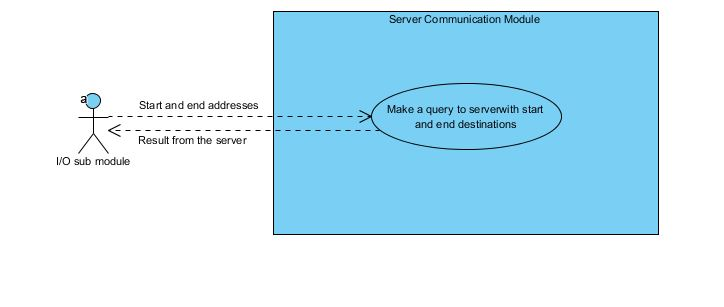
\includegraphics[scale=0.7]{grafiken/googleServerCommunication.jpg}
		\caption{Use case diagram: Google API sub-module communication}
		\label{fig:Google API communication}
	\end{figure}

	\par
	From the figure \ref{fig:Google API communication} it can be a seen that the API sub-module is 
	just an interface which communicates with the server to provide the calculated is a 
	middleware between the server and the navigation. 
	
	\section{Why I choose this package}
	The major focus of my objectives were related to the software engineering aspects instead of
	the hardware side. Personally I opted to go to this direction because I believe that software
	design is an important part of every project and it has always been a challenge to design a project base
	in a way which is robust, scalable and can be maintained with ease. By choosing this package,
	I had the flexibility to develop a system by applying the software design patterns and experiment with 
	the new	technologies available and see them in practice including, what are their pros and cons. 
	
%---------------------------------------------------------------------------------------------------	
% Second part of the thesis:
%---------------------------------------------------------------------------------------------------
	%---------------------------------------------------------------------------------------------------
% main part
%---------------------------------------------------------------------------------------------------
\newpage
%\part{main artl}
%---------------------------------------------------------------------------------------------------
% Analysis
%---------------------------------------------------------------------------------------------------
\newpage
\chapter{Requirement Analysis}
    The first phase of our project started off as a brainstorming stage where the functionality
    of the EGD was uncertain. Many discussions including a visit to the \textbf{dialog in the dark} 
    was conducted, where some questions were addressed to the visually impaired people to get an clear insight
    of what would they expect from EGD navigation system. 
\par
    From the discussions that were carried out, the requirements for the direction server were
    categorized into non-functional and functional parts which are mentioned below.
    
    \section{Functional Requirements}
        This section gives a detailed description of the functional aspects of the my work package % put a reference to this section
        and the direction API server in a tabular format in section \ref{ssec:FuncList}.
        \subsection{Functional requirements description}
            \label{ssec:FuncList}
            \begin{table}[h!]
                \centering
                    \begin{tabular}{|p{1cm}||p{15cm}|}
                        \hline
                            \textbf{No.} & \textbf{Requirement} \\
                        \hline
                            1. & Choose an appropriate operating system for the raspberry pi3 for implementing 
                            the navigation module i.e. raspbian \cite{raspbien}, 
                            android things \cite{androidThings} etc.\\
                        \hline
                            2. & Choose a software Architecture i.e. MVC \cite{mvc}, MVP \cite{mvp}
                            etc. to support the further development process.\\ 
                        \hline
                            3. & Choose an API which calculates the routes for the navigation i.e. Google Direction API \cite{googleDirecAPI}, mapbox \cite{mapbox} \\     
                        \hline
                            4. & Make an interface which can communicate to the API and return the result with a 
                            timeout to the server of 10s max, so that user gets immediate feedback. \\    
                        \hline  
                            5. & Apply Inversion of control container and use dependency Injection 
                            \cite{Martinfowler2014} framework to decouple the  dependencies 
                            in the project.\\
                        \hline   
                            6. & Run edge test cases to the API interface so that it can handle
                            errors.\\    
                        \hline    
                    \end{tabular}
                    \caption{List of functional requirements}
                    \label{table:functionalRequirements}
            \end{table}  

    \section{Non-functional Requirements}
        The requirements specified in this section present us the non-functional aspects of the 
        direction server. A tabular description is given below in the subsection 
        \ref{ssec:nonFuncList}. The detailed description depicts the benchmarks of how the system
        should be designed to meet the needs for a better sustainable prototype.

        \subsection{Non-Functional requirements description}
            \label{ssec:nonFuncList}
            \begin{table}[h!]
                \centering
                    \begin{tabular}{|p{0.5cm}||p{3cm}|p{11cm}|}
                        \hline
                            \textbf{No.} & \textbf{Requirement} & \textbf{Description} \\
                        \hline
                            1. &  Reliability & The system should provide the
                            correct walking routes. It should always take you through safe paths for 
                            walking.\\
                        \hline
                            2. & Usability & The system should be easy to use. This means the routes can be
                            calculated with just some simple parameters like start and end destination request.\\
                            
                        \hline
                            3. & Scalability & The server should be able to deal well with increase of use by many user,
                            and requesting new additional parameters i.e. change the return data to German etc., 
                            should not break the system.\\    
                        
                        \hline
                            4. & Maintainability & This relates to how the program is written and it 
                            should be designed using the software design patterns. So that it is easier to
                            debug and extend the app later.\\
                        \hline    
                            5. & Modifiability & It could be the case that the server chosen does not 
                            fulfill the use case later and the system should be decoupled.\\
                        \hline
                            6. & Responsiveness & The server should give some kind of feedback to the user
                            never the less if request cannot be made by providing an error log in case of
                            failure\\
                        \hline
                            7. & Migration of the app & Currently the proposal of the navigation module is to be
                            developed in a raspberry pi 3  and make it easier to port to a mobile device.\\ 
                                 
                        \hline    
                    \end{tabular}    
                \caption{List of non-functional requirements}
                \label{table:nonfunctionalRequirements}
            \end{table}   
						% chapter 2: Analysis
%---------------------------------------------------------------------------------------------------
% Design
%---------------------------------------------------------------------------------------------------
\newpage
\chapter{Software Design}
    Following the requirements described in the section \ref{ssec:FuncList}, there are
    some decisions that must be taken to design a solution for this module. The choices
    made to design a solution for the modules are explained in detail in the sections below.
    
    \section{Choosing an Operating System}
        A raspberry pi is a small portable sized computer that has an ability to
        do powerful processing i.e. run applications etc. Just as any other computer
        it requires an OS to function. The device supports different
        types of operating systems like raspbian, Linux, Android things etc. I would like to 
        make a comparison between raspbian and android things in detail 
        and determine which OS fits best for our use case.

        \subsection{Raspbian}
            Raspbian is a free operating system, which is debian based specially optimized 
            for the Raspberry pi \cite{raspbien}. This is one of the most popular OS for
            the Raspberry pi hardware. 

        \subsection{Android Things}
            Android Things is a relatively new Operating system in the \textbf{IoT} 
            \cite{IoT} world. The operating system is developed by google, 
            which provides a new android framework APIs and allows you 
            to create rapid prototypes \cite{androidThings}. Figure 
            \ref{fig:aThingsOverview} gives an overview on the different 
            abstraction layers of Android Things. 
            \begin{figure}[htbp!]
                \centering 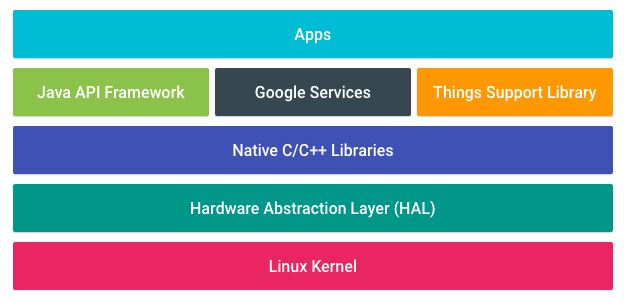
\includegraphics{grafiken/androidThingsOverview.jpg}
                \caption{Android Things OS Overview}
                \label{fig:aThingsOverview}
            \end{figure}
    
        
        \newpage
        \subsection{Comparison and Conlusion} 
            \label{ssec:OsComparison}  
            \begin{table}[h!]
                \centering
                \begin{tabular}{|p{9cm}|p{7.5cm}|}
                    \hline
                        \textbf{Android Things}  & \textbf{Raspbian}\\
                    \hline
                        Fast prototyping can be done because of the simplicity of setting
                        up a new project 
                        \url{https://developer.android.com/training/basics/firstapp/index.html}. & 
                        More development boards i.e. rpi2, raspberry pi zero etc. are supported\\
                    \hline
                        The existing android development tools, APIs and the huge resource library 
                        can be leveraged for easy development.
                        & It is more flexible in terms of what can be done since
                        it is an open-source OS.\\
                    \hline
                        It has very easy to use API's to connect to the development hardware.
                        \url{https://developer.android.com/things/sdk/pio/index.html} & Great
                        community support since there are more users.\\
                    \hline
                        Managing dependencies is very easy because the android development 
                        architecture is being used. It uses gradle to maintain the dependencies.
                        \url{https://gradle.org/}. & The OS is optimized for efficient use for
                        raspberry pi hardware.\\  
                    \hline
                \end{tabular}
                \caption{Comparision between Android Things and Raspbian}
                \label{table:aThingsVsRaspbian}     
        \end{table}

        \newpage 
        \par
            Both the operating systems have their own advantages and it would be biased to state that
            one of them is better than the other. After careful consideration and research, I
            decided to design the navigation module with Android Things which use Java as its
            programming language. The reasons why I choose android over raspbian are as follows:
            \begin{enumerate}
                \item 
                    Good and easy to understand documentation of how to setup 
                    a new project.
                \item 
                    Familiarity with the android and Java environment which increased my
                    productivity level.  
                \item 
                    The App written for the raspberry pi is similar to how one would
                    do it for native android so porting the app later to a native android
                    app if wanted would not be an issue. 
                \item 
                    The Java programming language has been around for a long time and many
                    frameworks to implement the software design patterns are readily 
                    available.
                \item 
                    The android environment makes it easy to handle dependencies using gradle
                    dependency manager, which is universal to all android packages. So the 
                    dependencies managing is not a issue if someone new installs the project.  
                \item
                    It has sample code examples for available APIs in github 
                    \url{https://developer.android.com/things/sdk/samples.html}. 
                \item
                    Android has a lot of frameworks which makes it easier to interface with an
                    external server via HTTP request \cite{http}.
            \end{enumerate}




							% chapter 3: Design
%---------------------------------------------------------------------------------------------------
% Realisation
%---------------------------------------------------------------------------------------------------
\newpage
\chapter{Implementation}
    \newpage
\section{Google API Service Implementation}
    Following the design in the section \ref{ssec:srp} the class 
    GoogleAPIService is responsible to make the request to the Google
    Direction API and return the result to the presenter which will be
    processed by the I/O service. The fig \ref{fig:directionServiceSeqDiagram}
    describes the object interactions and the messages exchanged during the
    single request that is made in order to receive a navigation data as described in
    the list \ref{code: googleAPi Result}.
    
    \par
        The GoogleDirectionAPIService implementation can be seen in
        the appendix \ref{code:googleAPIService}.
        Dependencies for the realizations are described below:
        \begin{enumerate}
            \item  
                \textbf{AsyncTaskUtil}
                    This is a custom made class which is reusable and used for background
                    operations see appendix \ref{code:AsyncUtil}. It is used here to make an HTTP request and this enables
                    the task to run without blocking the main thread. 
            \item  
                \textbf{GoogleDirectionApiMiddleware}
                As described earlier to make http request a HTTP client 
                is required and Retrofit
                is being used. Some parameters like the base endpoint of googleAPI 
                (where the http
                request would be made. i.e. https://maps.googleapis.com/), 
                connection and read timeouts
                to ensure the request is terminated 
                in case of situation when the server is not available 
                and error handling methods are configured in 
                GoogleDirectionMiddleware. Please see the appendix 
                \ref{code:retrofitConfig} to check the configuration. 
            \item  
                \textbf{DirectionAPI}
                    This is the model of the returned result from the Google
                    API.
            \item  
                \textbf{IAsyncTaskListenerOnFinish}
                    This is the listener which would get triggered when the
                    async task (HTTP request to Google API here) completes to
                    return the result.
        \end{enumerate}       
        



    \begin{figure}[htbp!]
        \centering 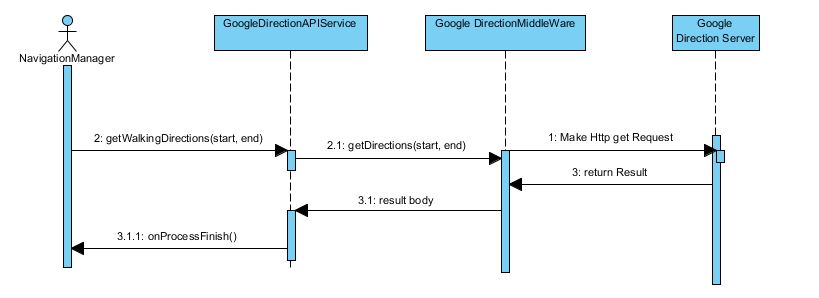
\includegraphics[scale=0.75]{grafiken/seqDigGoogleAPI.jpg}
        \caption{Sequence Diagram: Describing the functonality of the Google API service}
        \label{fig:directionServiceSeqDiagram}
    \end{figure}
    \newpage
\section{Dependency Injection With Dagger}
    \label{sec:daggerDIImplementation}
    This section is focused in explaining how dependency injection is implemented
    using the framework Dagger.
    The \url{https://github.com/slidenerd/Vivz_Dagger_2_Demo} has demos and snippets
    of how to add dagger as dependency to your project. There are three steps considered
    to achieve dependency Injection using dagger. The described procedure is the most
    basic steps needed. 
    \begin{enumerate}
        \item 
            \textbf{Create a class which defines what objects will be injected(Module)}
                Section \ref{code:moduleDaggerExample} shows an example of class which instantiates 
                objects which would be injected. @Module defines the class and @Provides
                defines the method which provide the dependencies to be injected. Without the
                @Provides annotation the object will not be injected. 
                It is best practice to make the modules small, and only define 
                the objects in the a here 
                which belong together i.e. NetworkCheckUtilModule would only have
                objects that NavigationCheck class would require.  
        \item 
            \textbf{Create a Component class}
                A component(@Component) is an interface for dagger where one  must define 
                what modules to choose and which class should these dependencies be injected into. 
                Appendix \ref{code:componentDaggerExample} shows an example of the implementation of a 
                component class.
                Through the inject method you define
                which classes receive the dependencies. A Component class can contain 
                many modules, this is done so that the modules could be reusable. 
        \item 
            \textbf{Inject the dependencies}
                The last thing to be done is to inject the dependencies. This is done by
                using the annotation @Inject and then in the constructor run the builder
                of the corresponding component see Appendix \ref{code:injectionDaggerExample} for the
                implementation. 
    \end{enumerate}
    For more detailed information for the annotations check out
    this \url{http://www.vogella.com/tutorials/Dagger/article.html}.
    













	% Chapter 4: Realisation

%---------------------------------------------------------------------------------------------------
% Thrd art of the thesis
%---------------------------------------------------------------------------------------------------
	%---------------------------------------------------------------------------------------------------
%end
%---------------------------------------------------------------------------------------------------
\newpage
%\part{end}
\chapter{Conclusion}
The last important words...
																								
%---------------------------------------------------------------------------------------------------	
%references
%---------------------------------------------------------------------------------------------------		

\renewcommand{\bibname}{References}
\bibliographystyle{abbrv}       		    														% passed to German reference organisation
                                          														% Alphabetic sorting, abbreviations
  \bibliography{literatur/literatur}      														% reference list
  % references added but need not be referenced inside the text
% references used inside the text with  \nocite or \cite must be added to the .bib File!

%\nocite{Guenther:2002}
%\nocite{Lamport:1995}
%\nocite{Goossens:2000}
%\nocite{Kohm:2003}
%\nocite{Hunt:2003}
%\nocite{Boehm:2002}
%\nocite{Schmatz:2004}
%\nocite{Streitz:2005}
%\nocite{HP:2004}
%\nocite{Luede:2004}
%\nocite{Demarco:1999}
%\nocite{Kollakowski:2004}
%\nocite{Dawson:2003}
%\nocite{Poenicke:1988}
%\nocite{Kruse:2000}
%\nocite{Nilsson:1998}
%\nocite{Heinsohn:1999}
%\nocite{Luger:2001}
%\nocite{Kuehnel:2001}
%\nocite{Bigus:2001}
%\nocite{Ferber:2001}
%\nocite{Wooldridge:2002}
%\nocite{KuroseRoss:2002}
%\nocite{Vogt:2001}
%\nocite{Roetzer:1999}
%nocite{P3P:2004}
%\nocite{CPEX:2004}
%\nocite{Duden:1997}
%\nocite{Hoerauf:2001}
%\nocite{Schirru:2004}
%\nocite{Babic:2003}
%\nocite{Luepke:2004}

\nocite{googleDirecAPI}
\nocite{rpi3}
\nocite{mvc}
\nocite{mvp}
\nocite{mapbox}
\nocite{raspbien}
\nocite{androidThings}
\nocite{Martinfowler2014}
\nocite{IoT}
\nocite{http}
\nocite{Hotop2015}
\nocite{Potel}
\nocite{AdamCarlson}
\nocite{Gradle}
\nocite{GoogleIO}
\nocite{GoogleStart}
\nocite{GoogleWebServices}
\nocite{MicrosoftMVC}
\nocite{JavaSpring}
\nocite{TinMegali2016}
\nocite{Codepath}
\nocite{Pivotal}
\nocite{GoogleAsync}
\nocite{Square}
\nocite{SquareDagger}
\nocite{AkhileshGoveeshSEECHURN}
																				%add the non refeenced papers or literature which are as well important for the thesis!

  \chapter{Appendix}
    \begin{figure}[htbp!]
        \centering 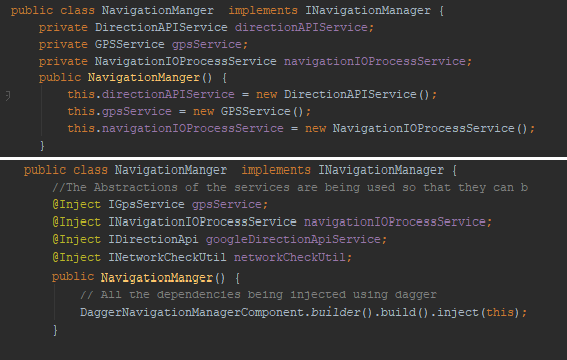
\includegraphics{grafiken/di_compare.png}
        \caption{Comparision of code with(bottom) and without Dependency injection(bottom)}
        \label{fig:DIComparision}
    \end{figure}
%---------------------------------------------------------------------------------------------------	
% appendix
%---------------------------------------------------------------------------------------------------	
	\appendix
% \input{anhang/hilfsmittel/hilfsmittel}															% appendix A: helps for the implementation
																																			% 					of this thesis
%	\input{anhang/quellcode/quellcode}																	% Appendix B: SourceCode

%---------------------------------------------------------------------------------------------------	
% Glossar
%---------------------------------------------------------------------------------------------------	
	\printnomenclature

%---------------------------------------------------------------------------------------------------	
% index
%---------------------------------------------------------------------------------------------------	
	\printindex
	
%---------------------------------------------------------------------------------------------------	
% Declaration
%---------------------------------------------------------------------------------------------------		
	\asurency	

%--------------------------------------------------------------------------------------------------- 
% End of the thesis
%--------------------------------------------------------------------------------------------------- 
\end{document}
